\documentclass[12pt]{article}
\usepackage[margin=1in]{geometry}
\usepackage{array}
\usepackage{graphicx}
\usepackage{longtable}

\pagenumbering{gobble}

\graphicspath{{./plots/}}

\begin{document}
 \begin{center}
  \huge{\textbf{CIFAR-10 Image Classification}\\}
  \Large{CSE471 - Statistical Methods in AI}\\
  Mini-project-2\\
  \vspace{0.2in}
  Karnik Ram\\
  2018701007
 \end{center}
 
\section*{Introduction}

Four classifiers - Multi-layer Perceptron, Linear Support Vector Machine, Nonlinear Support Vector Machine, and Logistic Regression were tested for classification task on the CIFAR-10 dataset. Details of the techniques used during the training process are described, followed by the results for each classifier.

\section*{Dataset}

The dataset contains $60,000$ RGB images from 10 classes, each of dimensions $32 \times 32$. There are $6,000$ images per class. The training set contains $50,000$ images and the test set contains $10,000$ images. The training set is split into $5$ batches, however the number of images per category varies across the batches. So to avoid any bias, all the batches are appended together and randomly sampled to form batches where ever needed in my experiemnts. The test set contains exactly $1,000$ images per class.

Each image is stored as a $3072$ vector, with values between $[0,255]$. This raw representation is used as such to obtain baseline scores for all the classifiers before preprocessing.

\section*{Data Preprocessing}

Four different techniques were tested to help with classification accuracy and runtime.

\subsection*{Feature scaling}

In this technique, the feature values are linearly scaled to the range $[0, 1]$. This scaling can help avoid values in higher ranges dominating those in smaller ranges. This also helps avoid numerical difficulties during the calculations.

\subsection*{Mean Subtraction}

In this technique, the samples are zero-centered by subtracing the mean from every sample. The mean is computed only for the train samples and then subtracted from all the train/test samples. This helps improve the learning process by making the sample values to be both positive and negative.

\subsection*{Principal Component Analysis}

Principal Component Analysis (PCA) is a linear dimensionality reduction algorithm used to obtain a lower dimensional representation of the original feature vectors, while retaining maximum variance. While this doesn't cause much increase in accuracy, it does result in significant speed-up of the downstream algorithms. The configurable value is the number of components, $k$, which was chosen such that the explained variance ratio is at least $0.9$. For the CIFAR-10 dataset, this was found to be $99$.

\subsection*{Linear Discriminant Analysis}
Linear Discriminant Analysis (LDA) is a linear dimensionality reduction algorithm that is also disrciminative in nature. It maximizes the separation between the classes while minimizing the intra-class variation, which results in better accuracy for the downstream classifiers. The maximum number of components is equal to \textit{numclasses - 1}, which is what was chosen for all the experiments.

\vspace{1em}
\noindent All of these different pre-processing options were tried out by passing optional arguments to the programs as described in the README.

\section*{Training}

The entire training set of $50,000$ samples was used for the training process after appropriate preprocessing. A smaller subset was used for the hyperparameter search as described below.

\subsection*{Choosing Hyperparameters}

Each of the classifiers used has a set of hyperparameters that have to be set outside of the learning process. The multi-layer peceptron has the maximum number of hyperparameters, while linear svm and non-linear svm have the least.

Hyperparameters can be set manually or can be found using automatic search algorithms like grid search and random search. In order to tune manually one must properly understand the relationship between each hyperparameter and the model's performance. Instead, grid search is done by training the model for every possible comination of hyperparameter values from a finite set of user-provided values for each hyperparameter, and then choosing the one that achieves best performance. Random search is a faster alternative to grid search, where the probabililty distributions of the individual hyperparamters are to be provided which are then randomly sampled.

Grid search was used in my experiments to find the optimal value of hyperparameters. Only a small randomly sampled subset of the training set ($5000$ samples) in raw representation form were used for grid search in the interest of computation time. Since the size of the validation set is small, to obtain a less noisy estimate of the hyperparamters, 5-fold cross-validation was used. Here, the subset was split into $5$ equal folds, $4$ for training, and $1$ for validation, and the validation fold was chosen iteratively over all the folds. The mean of the error over all the validation folds was used to determine the best choice of hyperparameters. 

Both grid search and cross validation were implemented without using any libraries. \texttt{accuracy\_score} was used as the error metric during validation. The following were the hyperparameters that were tuned for each classifier.

\begin{center}
 \begin{tabular}{|c|m{10em}|}
 \hline
 Classifier & Hyperparameters \\
 \hline
 Multi-layer Perceptron & Number of layers (L), number of units per layer (U), learning rate (lr) \\
 \hline
 Linear SVM & Regularization factor (C) \\
 \hline
 Kernel SVM & Regularization factor (C), gamma\\
 \hline
 Logistic Regression & Regularization factor (C) \\
 \hline
 \end{tabular}
\end{center}

\subsection*{Overfitting}

Overfitting occurs when the gap between the train error and test error is too large. This is determined by the model's capacity, or its ability to fit a range of functions. Models with low capacity tend to underfit or have high train error while models with high capacity tend to ``memorize'' the properties of the train set and hence perform poorly on the test set.

For instance, in the case of MLP this occurs when the number of layers is too large that the model begins to tightly fit the train data and attain very low train error. An example of this is shown below.

\begin{center}
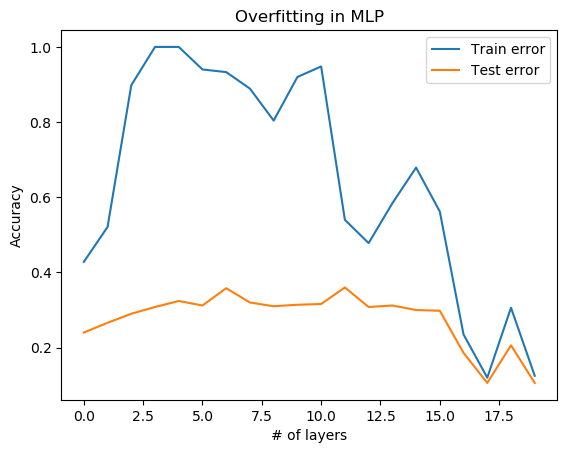
\includegraphics[scale=0.5]{mlp-overfit.png}
\end{center}

We avoid overfitting by limiting the representational capacity of the model, in the case of MLP this would be the number of layers, and by introducing regularizer terms to increase the preference for certain kind of functions.
\section*{Results}

\subsection*{Multi-layer Perceptron}
A multi-layer perceptron was implemented using the \texttt{MLPClassifier} class in sklearn. The model uses the adam solver and runs for $200$ epochs by default. Early stopping was not used. The accuracy score of the default model with one hidden layer and 100 hidden units, and learning rate equal to $0.001$ was found to be $0.099$.

The number of hidden layers (L) and number of units per layer (U), specified by the \texttt{hidden\_layer\_sizes} argument was first tuned for using grid search. L was searched over the range $[1,2,3,4]$ and U over the range $[50,100,500,1000]$. 

\begin{center}
 %\begin{tabular}{|m{3em}|m{3em}|m{3em}|}
 \begin{tabular}{|c|c|c|}
  \hline
  L & U & Mean validation accuracy \\
  \hline
  1 & 50 & 0.103\\
  1 & 100 & 0.099\\
  1 & 500 & 0.1226\\
  1 & 1000 & 0.1548\\
  2 & 50 & 0.1656\\
  2 & 100 & 0.2664\\
  2 & 500 & 0.2996\\
  2 & 1000 & 0.2756\\ 
  3 & 50 & 0.235\\
  3 & 100 & 0.2726\\
  3 & 500 & 0.3132\\
  3 & 1000 & 0.3126\\ 
  4 & 50 & 0.2364\\
  4 & 100 & 0.3062\\
  4 & 500 & 0.3252\\
  \textbf{4} & \textbf{1000} & \textbf{0.3378}\\ 
  \hline
 \end{tabular}

\end{center}

The combination of $(4,1000)$ gave the best validation accuracy, and higher values for L did increase the accuracy but it also increased the computation time significantly and led to overfitting.

Next, after fixing \texttt{hidden\_layer\_sizes} to $4 * (1000,)$ the learning rate parameter controlled by the \texttt{learning\_rate\_init} argument was tuned. The best value was found to be $0.001$, although one could do a further fine search around that point.

\begin{center}
\begin{tabular}{|c|c|}
 \hline
 Learning rate & Mean validation accuracy \\
 \hline
 0.0001 & 0.3344\\
 \textbf{0.001} & \textbf{0.3444}\\
 0.01 & 0.1102\\
 0.1 & 0.1034\\
 1 & 0.1038\\
 \hline
\end{tabular}
\end{center}

\begin{center}
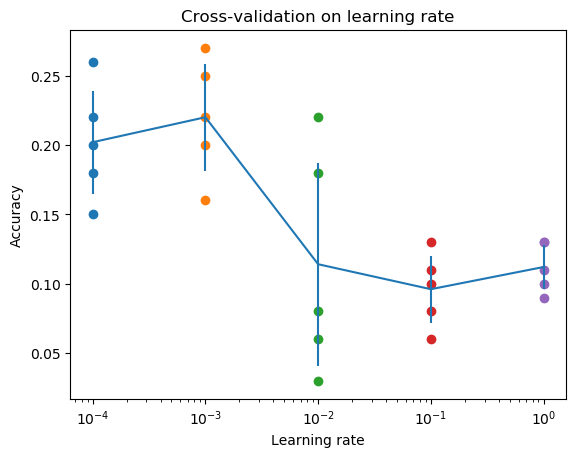
\includegraphics[scale=0.6]{mlp-lr.png}
\end{center}

Next, after fixing both the arguments to the found values, the model was tested with different feature representations. The results are as follows,

\begin{center}
  \begin{tabular}{|c|c|c|}
    \hline
    Representation & Accuracy & F1-score \\
    \hline
    Raw & 0.4695 & 0.4667\\
    Scaled & 0.4966 & 0.4933 \\
    Mean centered & 0.5259 & 0.5263\\
    PCA & 0.5026 & 0.5025\\
    LDA & 0.3149 & 0.3150 \\
    \hline
  \end{tabular}
\end{center}


\subsection*{Linear Support Vector Machine}

A linear support vector machine model was implemented using the \texttt{LinearSVC} class in sklearn. The model uses liblinear and the accuracy score of the default model was found to be $0.19$ with C equal to $1$.

The regularization parameter, C, which controls the trade-off between the complexity of the model and the number of non-separable points was then tuned. C was initially tested with arbitrary high values and low values and it seemed to perform better with low values, so the search range was chosen to be $[0.001,0.001,0.1,1,2,4]$.

\begin{center}
\begin{tabular}{|c|c|}
 \hline
 Regularization C& Mean validation accuracy \\
 \hline
 0.001 & 0.2234\\
 0.01 & 0.2196\\
 0.1 & 0.2172\\
 1 & 0.2206\\
 2 & 0.2186\\
 \textbf{4} & \textbf{0.2248}\\
 \hline
\end{tabular}
\end{center}

\begin{center}
 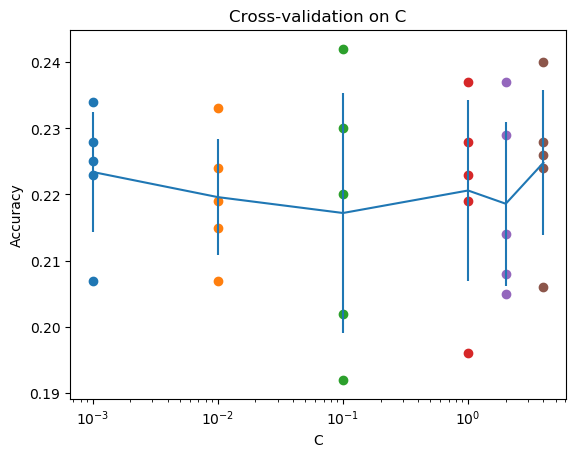
\includegraphics[scale=0.5]{lsvm-c.png}
\end{center}

Next, after fixing C to be equal to $4$, the model was tested with different feature representations. The results are as follows,

\begin{center}
  \begin{tabular}{|c|c|c|}
    \hline
    Representation & Accuracy & F1-score \\
    \hline
    Raw & 0.1954 & 0.1699\\
    Scaled & 0.2713 & 0.2357\\
    Mean centered & 0.2143 & 0.2161\\
    PCA & 0.1950 & 0.1837\\
    LDA & 0.3679 & 0.3617 \\
    \hline
  \end{tabular}
\end{center}

\subsection*{Non-linear Kernel Support Vector Machine}

A kernel SVM model was implemented using the \texttt{SVC} class in sklearn. The model uses the rbf kernel and is based on libsvm. The accuracy score of the default model was found to be $0.1477$.

The C parameter, and the $\gamma$ parameter of the rbf kernel are then tuned together using grid search. After initial testing the model was found to perform well for very small $\gamma$ values, so C was searched for over the range $[1,2,4,8]$ and $\gamma$ over the range $[10^{-9},10^{-8},10^{-7},10^{-6}]$.

\begin{center}
 %\begin{tabular}{|m{3em}|m{3em}|m{3em}|}
 \begin{longtable}{|c|c|c|}
  \hline
  C & $\gamma$ & Mean validation accuracy \\
  \hline
  1 & $10^{-9}$ & 0.2586\\
  1 & $10^{-8}$ & 0.3600\\
  1 & $10^{-7}$ & 0.4096\\
  1 & $10^{-6}$ & 0.1656\\
  2 & $10^{-9}$ & 0.2978\\
  2 & $10^{-8}$ & 0.3768\\
  \textbf{2} & \textbf{$10^{-7}$} & \textbf{0.4214}\\
  2 & $10^{-6}$ & 0.18\\
  4 & $10^{-9}$ & 0.3282\\
  4 & $10^{-8}$ & 0.3924\\
  4 & $10^{-7}$ & 0.4178\\
  4 & $10^{-6}$ & 0.18\\
  8 & $10^{-9}$ & 0.3478\\
  8 & $10^{-8}$ & 0.3962\\
  8 & $10^{-7}$ & 0.4110\\
  8 & $10^{-6}$ & 0.18\\
  \hline
 \end{longtable}

\end{center}

Kernel SVM seemed to be the most sensitive to hyperparameter changes. Next, after fixing C to be equal to $2$, and $\gamma$ equal to $10^{-7}$, the model was tested with different feature representations. The results are as follows,

\begin{center}
  \begin{tabular}{|c|c|c|}
    \hline
    Representation & Accuracy & F1-score \\
    \hline
    Raw & 0.5679 & 0.5673\\
    Scaled & 0.2529 & 0.2034\\
    Mean centered & 0.5679 & 0.5673\\
    PCA & 0.5560 & 0.5550\\
    LDA & 0.3473 & 0.3450\\
    \hline
  \end{tabular}
\end{center}

\subsection*{Logistic Regression}

A logistic regression model was implemented using the \texttt{LogisticRegression} class in sklearn. The lbfgs solver was used and the multi-class scheme was set to multinomial. The accuracy score of the default model was found to be $0.4024$, with C equal to $1$.

The C parameter was then tuned, and the best value was found to be $10^{-7}$.

\begin{center}
\begin{tabular}{|c|c|}
 \hline
 Regularization C& Mean validation accuracy \\
 \hline
  $10^{-9}$& 0.2460\\
 $10^{-8}$ & 0.3324\\
 $\mathbf{10^{-7}}$ & \textbf{0.3534}\\
 $10^{-6}$ & 0.3378\\
 $10^{-5}$ & 0.3230\\
 $10^{-4}$ & 0.3166\\
 $10^{-3}$ & 0.3164\\
 $10^{-2}$ & 0.3172\\
 $10^{-1}$ & 0.3182\\
 $1$ & 0.3192\\
 \hline
\end{tabular}
\end{center}

\begin{center}
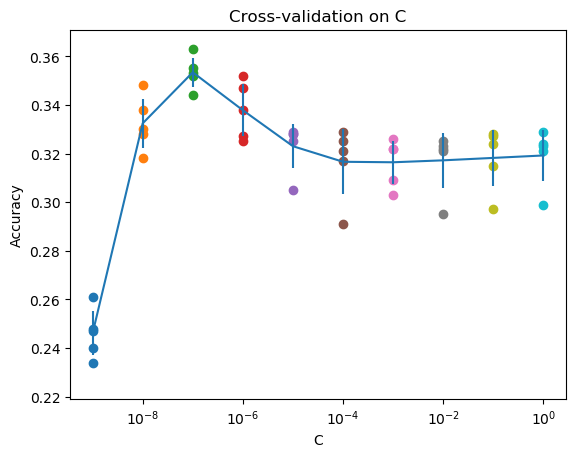
\includegraphics[scale=0.6]{lreg-c.png}
\end{center}

Logistic regression model seemed to have the quickest runtime among all. After setting C to be equal to $10^{-7}$, the model was tested with different feature representations. The results are as follows,

\begin{center}
  \begin{tabular}{|c|c|c|}
    \hline
    Representation & Accuracy & F1-score \\
    \hline
    Raw & 0.4041 & 0.4002\\
    Scaled & 0.2540 & 0.2026 \\
    Mean centered & 0.4130 & 0.4055\\
    PCA & 0.4044 & 0.3926\\
    LDA & 0.3684 & 0.3565 \\
    \hline
  \end{tabular}
\end{center}

Clearly, neither the hyperparameter search nor the data preprocessing seemed to have had any great improvement to the default model performance.

\end{document}
